\section{Results}

\subsection{Evaluation of Existing Models}
We evaluated IACA, llvm-mca, Ithemal\cite{ithemal}, and OSACA\cite{osaca}
on three recent Intel microarchitectures: Ivy Bridge, Haswell, Skylake.
Some basic blocks in our dataset contains AVX2 instructions, which are not supported in Ivy Bridge,
and these basic blocks are not included in validation for Ivy Bridge.
We use relative error (i.e. absolute error of the predicted throughput normalized by the measured throughput)
as the metric to measure inaccuracy.
Table \ref{tab:overall} shows the unweighted average error
of each model on different microarchitectures.
% include ivb and skl
Figures \ref{fig:ivb-app-err}, \ref{fig:hsw-app-err}, and \ref{fig:skl-app-err}
show the breakdown of the errors by applications.
Figure \ref{fig:ivb-cluster-err}, \ref{fig:hsw-cluster-err}, 
and \ref{fig:skl-cluster-err} show the breakdown of the errors by basic block categories 
(see \ref{classification} for details of basic blocks classification).
We note that the overall error of each model can be unrepresentative
of its performance on a given domain.
The discrepancy between these models' overall unweighted accuracy
and that of specialized domains (e.g. numerical kernels) highlights
the need of basic block classification and per-class error reporting.

Generally speaking, basic blocks dominated by stores
(category-4) are easier to predict,
while the throughput of basic blocks that mixes load instructions
with other operations (e.g. category-8) are considerably
more difficult to predict -- the prediction error is on average more than
twice higher than predicting basic blocks with only stores. 
We surmise that this is due to weakness of existing analyzers to model 
memory dependence.
In addition to basic blocks with memory dependence,
vectorized basic blocks (e.g. category-2) also causes high prediction errors.

% TODO summarize error by applications

\textbf{IACA}~\cite{iaca} is relatively more stable compared to other models that we evaluated.
An interesting point to note is that IACA is consistently accurate on basic blocks from OpenSSL.

\textbf{llvm-mca} is on par with IACA on Ivy Bridge and Haswell but considerably worse on Skylake,
especially on modelling basic blocks involving basic arithmetic operations.
We suspect the decrease in performance in Skylake is a result of LLVM developers 
having less time updating the cost models for the relatively new microarchitecture.

\textbf{Ithemal}~\cite{ithemal} consistently outperforms other models, except on vectorized basic blocks (i.e. category-2).
Ithemal is also considerably better than other models at modelling basic blocks with memory dependence,
as demonstrated by its errors on predicting basic blocks from categories 4 and 8.
We discussed ithemal's underformance on vectorized basic blocks with the authors of Ithemal, who suggested that the inconsistency
was a result of imbalance in their training dataset;
the majority of which, similar to our data set, consists of non-vectorized basic blocks.
In addition, the authors of Ithemal reported having to leave more basic blocks out of the training of their
Skylake model due to lack of reliable throughput measurements.
% TODO comapre error to basic block length and show ithemal does not generalize to large baisc blocks

\textbf{OSACA}\cite{osaca} generally has higher errors compared to other models.
We note that this might have less to do with OSACA's methodology than the engineering of its instruction parser.
During our evaluations, we found and reported five bugs related to OSACA's instruction parser.
In particular, OSACA does not recognize several instruction forms;
depends on the cases, it either crashes or treats unrecognized instruction forms as nops.
One such instruction form is any instruction that reads an immediate operand and writes to memory
(e.g. \verb|add [rbx], 1|), and OSACA treats these instructions as nops, thus under-reporting the throughput of
many basic blocks.


\begin{table}
\begin{tabular}{|p{0.25\columnwidth}|p{0.3\columnwidth}|p{0.25\columnwidth}|}
\hline

Microarchitecture & Model & Average Error\\
\hline

Ivy Bridge & IACA & 0.1693\\
    & llvm-mca & 0.1885\\
    & Ithemal & 0.1180\\
    & OSACA & 0.3277\\
\hline

Haswell & IACA & 0.1798\\
    & llvm-mca & 0.1832\\
    & Ithemal & 0.1253\\
    & OSACA & 0.3916\\
    
\hline 
Skylake & IACA & 0.1578\\
    & llvm-mca & 0.2278\\
    & Ithemal & 0.1191\\
    & OSACA & 0.3768\\

\hline
% TODO more for IVB and SKL
\end{tabular}
\\
\caption{Overall error of evaluated models.}
\label{tab:overall}
\end{table}

\begin{figure}
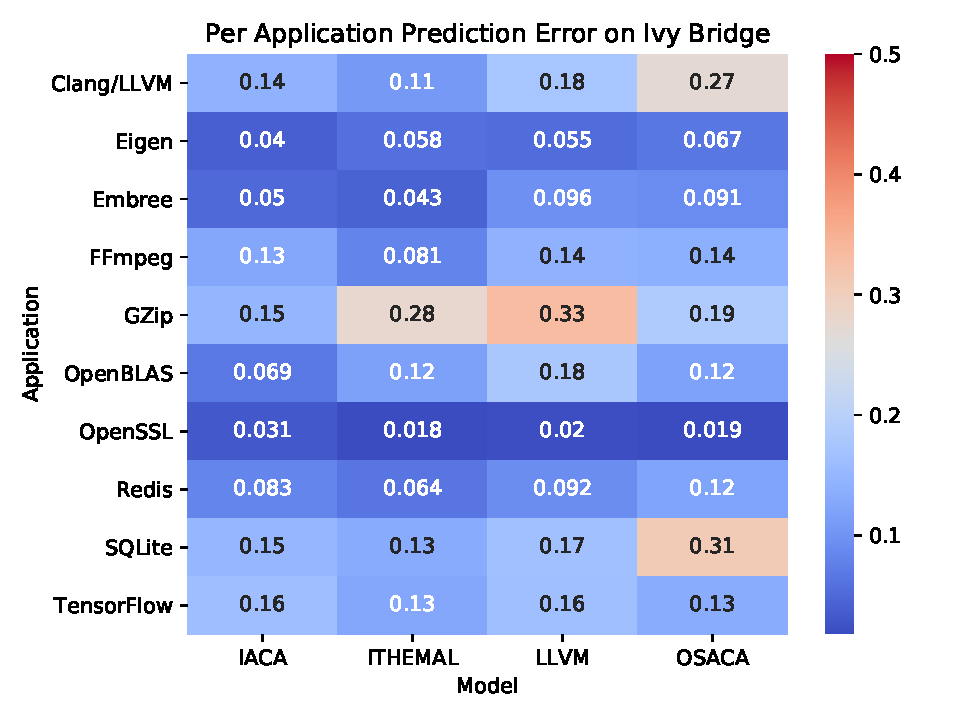
\includegraphics[width=\columnwidth]{figures/ivb-app-err.pdf}
\caption{Per-application error for each model on Ivy Bridge;
error for each basic block is weighted by the frequency it is sampled during profiling.}
\label{fig:ivb-app-err}
\end{figure}

\begin{figure}
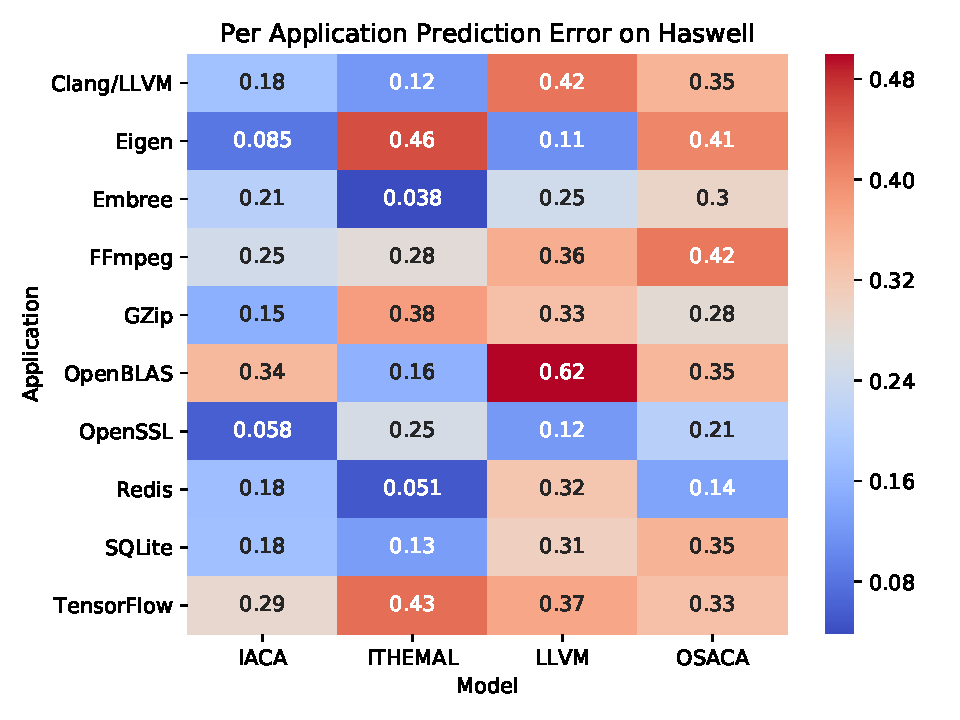
\includegraphics[width=\columnwidth]{figures/hsw-app-err.pdf}
\caption{Per-application error for each model on Haswell}
\label{fig:hsw-app-err}
\end{figure}

\begin{figure}
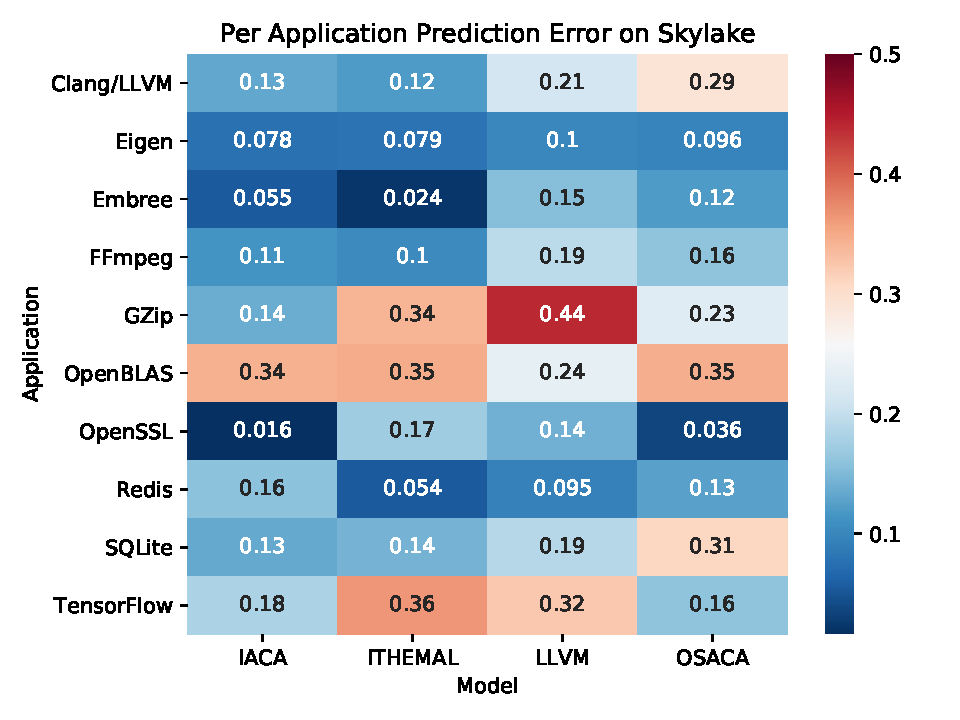
\includegraphics[width=\columnwidth]{figures/skl-app-err.pdf}
\caption{Per-application error for each model on Skylake. }
\label{fig:skl-app-err}
\end{figure}

\begin{figure}
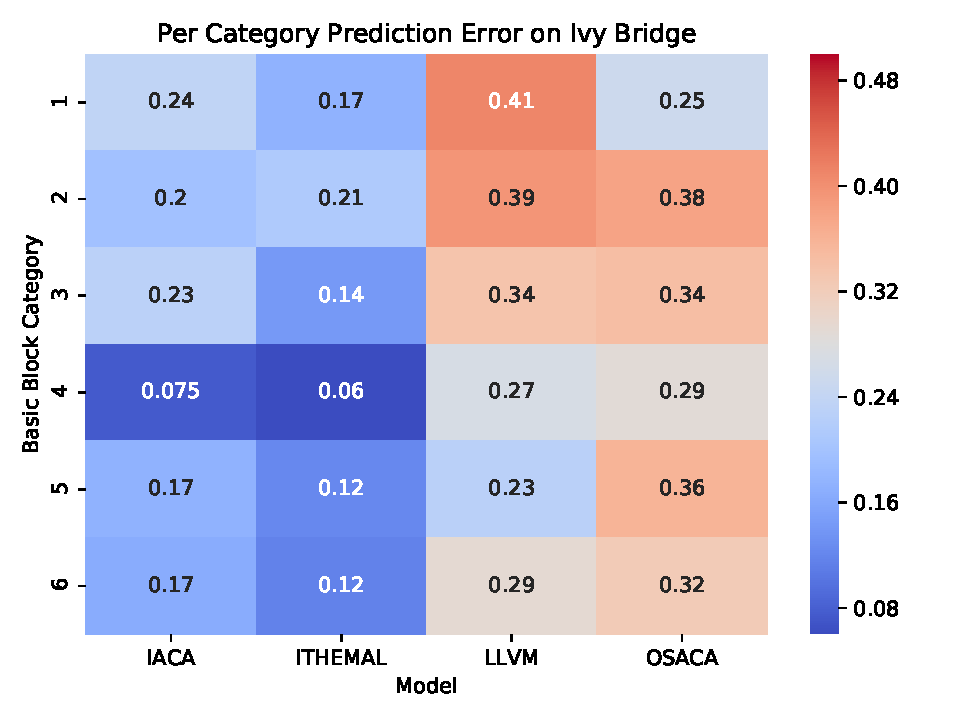
\includegraphics[width=\columnwidth]{figures/ivb-cluster-err.pdf}
\caption{Per-cluster error for each model on Ivy Bridge}
\label{fig:ivb-cluster-err}
\end{figure}

\begin{figure}
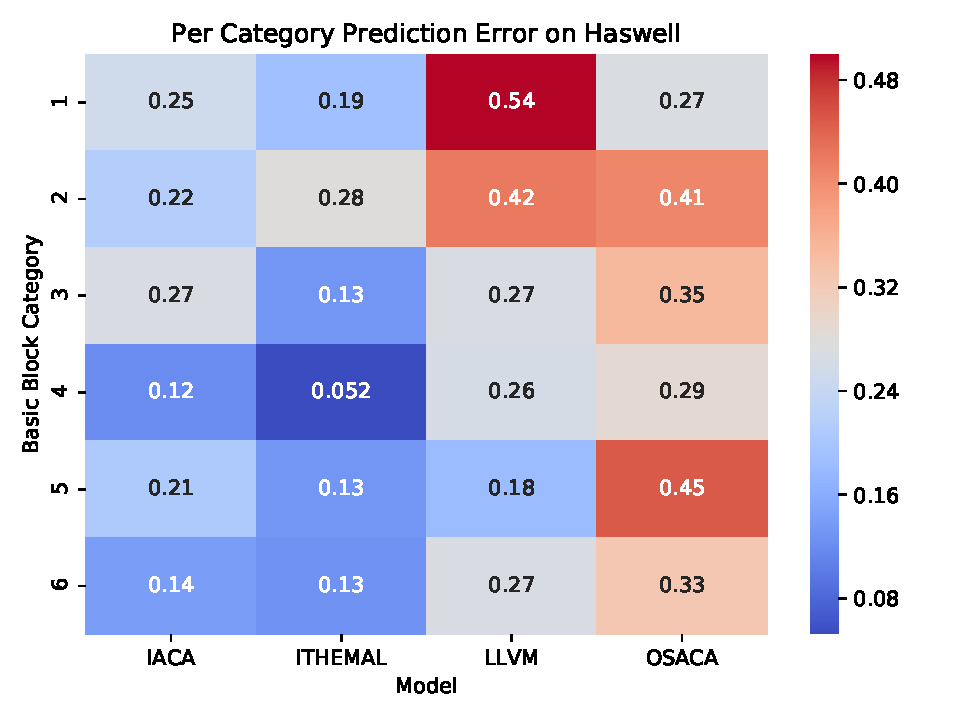
\includegraphics[width=\columnwidth]{figures/hsw-cluster-err.pdf}
\caption{Per-cluster error for each model on Haswell}
\label{fig:hsw-cluster-err}
\end{figure}

\begin{figure}
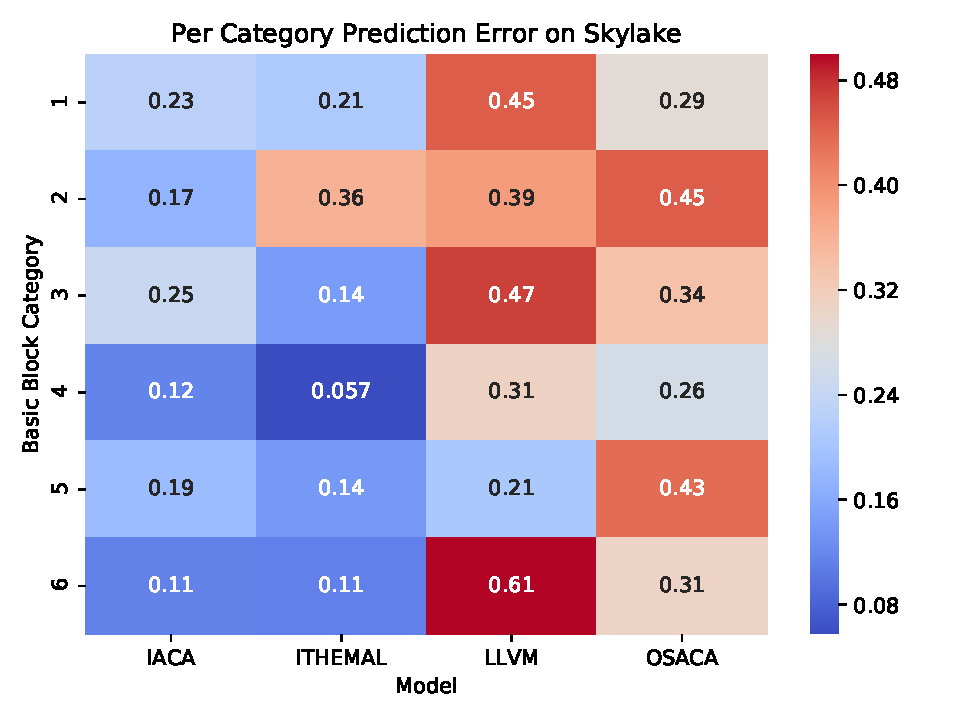
\includegraphics[width=\columnwidth]{figures/skl-cluster-err.pdf}
\caption{Per-cluster error for each model on Skylake}
\label{fig:skl-cluster-err}
\end{figure} 
